%   DOCUMENT CLASS  %%%%%%%%%%%%%%%%%%%%%%%%%%%%%%%%%%%%%%%%%%%%%%%%%%%%%%%%%%%
%
%   Use the `sfuthesis` class to format your thesis. If your program does not
%   require a thesis defence, use the class option `undefended` like so:
%
%     \documentclass[undefended]{sfuthesis}
%
%   To generate a signature page for your defence, use the `sfuapproval` class
%   instead, by replacing the below line with
%
%     \documentclass{sfuapproval}
%
%   For more information about thesis formatting requirements, go to
%
%     http://www.lib.sfu.ca/help/publish/thesis
%
%   or ask a thesis advisor at the SFU Research Commons.
%

\documentclass{sfuthesis}



%   DOCUMENT METADATA  %%%%%%%%%%%%%%%%%%%%%%%%%%%%%%%%%%%%%%%%%%%%%%%%%%%%%%%%
%
%   Fill in the following information for the title page and approval page.
%

\title{An example of a thesis or dissertation on the subject of your degree}
\thesistype{Dissertation}
\author{Amirali Sharifian}
\previousdegrees{%
	M.Sc., Simon Fraser University, 2016\\
	B.Sc., Isfahan University of Technology, 2014}
\degree{Doctor of Philosophy}
\discipline{Computer Science}
\department{Department of Computing Science}
\faculty{Faculty of Mad Science}
\copyrightyear{2019}
\semester{Summer 2019}
\date{January 10, 2017}

\keywords{thesis template; Simon Fraser University; time travel paradoxes}

\committee{%
	\chair{Pamela Isely}{Professor}
	\member{Emmett Brown}{Senior Supervisor\\Professor}
	\member{Bonnibel Bubblegum}{Supervisor\\Associate Professor}
	\member{James Moriarty}{Supervisor\\Adjunct Professor}
	\member{Kaylee Frye}{Internal Examiner\\Assistant Professor\\School of Engineering Science}
	\member{Hubert J.\ Farnsworth}{External Examiner\\Professor\\Department of Quantum Fields\\Mars University}
}



%   PACKAGES %%%%%%%%%%%%%%%%%%%%%%%%%%%%%%%%%%%%%%%%%%%%%%%%%%%%%%%%%%%%%%%%%%
%
%   Add any packages you need for your thesis here.
%   You don't need to call the following packages, which are already called in
%   the sfuthesis class file:
%
%   - appendix
%   - etoolbox
%   - fontenc
%   - geometry
%   - lmodern
%   - nowidow
%   - setspace
%   - tocloft
%
%   If you call one of the above packages (or one of their dependencies) with
%   options, you may get a "Option clash" LaTeX error. If you get this error,
%   you can fix it by removing your copy of \usepackage and passing the options
%   you need by adding
%
%       \PassOptionsToPackage{<options>}{<package>}
%
%   before \documentclass{sfuthesis}.
%
%   The following packages are a few suggestions you might find useful.
%
%   (1) amsmath and amssymb are essential if you have math in your thesis;
%       they provide useful commands like ``blackboard bold'' symbols and
%       environments for aligning equations.
%   (2) amsthm includes allows you to easily change the style and numbering of
%       theorems. It also provides an environment for proofs.
%   (3) graphicx allows you to add images with \includegraphics{filename}.
%   (4) hyperref turns your citations and cross-references into clickable
%       links, and adds metadata to the compiled PDF.
%   (5) pdfpages lets you import pages of external PDFs using the command
%       \includepdf{filename}. You will need to do this if your research
%       requires an Ethics Statement.
%

\usepackage{amsmath}                            % (1)
\usepackage{amssymb}                            % (1)
\usepackage{amsthm}                             % (2)
\usepackage{graphicx}                           % (3)
\usepackage[pdfborder={0 0 0}]{hyperref}        % (4)
\usepackage{minted}
% \usepackage[outputdir=cache]{minted}
\usepackage{filecontents}
% \usepackage{natbib}
\usepackage{bibentry}
\usepackage{xcolor}

\nobibliography*

\definecolor{LightGray}{gray}{0.9}
%\definecolor{DarkGray}{gray}{0.1}

%\pagecolor{DarkGray}

% \usemintedstyle{borland}

%New colors defined below
\definecolor{codegreen}{rgb}{0,0.6,0}
\definecolor{codegray}{rgb}{0.5,0.5,0.5}
\definecolor{codepurple}{rgb}{0.58,0,0.82}
\definecolor{backcolour}{rgb}{0.95,0.95,0.92}

% \usepackage{pdfpages}                         % (5)
% ...
% ...
% ...
% ... add your own packages here!




%   OTHER CUSTOMIZATIONS %%%%%%%%%%%%%%%%%%%%%%%%%%%%%%%%%%%%%%%%%%%%%%%%%%%%%%
%
%   Add any packages you need for your thesis here. We've started you off with
%   a few suggestions.
%
%   (1) Use a single word space between sentences. If you disable this, you
%       will have to manually control spacing around abbreviations.
%   (2) Correct the capitalization of "Chapter" and "Section" if you use the
%       \autoref macro from the `hyperref` package.
%   (3) The LaTeX thesis template defaults to one-and-a-half line spacing. If
%       your supervisor prefers double-spacing, you can redefine the
%       \defaultspacing command.
%

\frenchspacing                                    % (1)
\renewcommand*{\chapterautorefname}{Chapter}      % (2)
\renewcommand*{\sectionautorefname}{Section}      % (2)
\renewcommand*{\subsectionautorefname}{Section}   % (2)
% \renewcommand{\defaultspacing}{\doublespacing}  % (3)
% ...
% ...
% ...
% ... add your own customizations here!


%% Include command tex file
\def\code#1{\texttt{#1}}


%   FRONTMATTER  %%%%%%%%%%%%%%%%%%%%%%%%%%%%%%%%%%%%%%%%%%%%%%%%%%%%%%%%%%%%%%
%
%   Title page, committee page, copyright declaration, abstract,
%   dedication, acknowledgements, table of contents, etc.
%
%   If your research requires an Ethics Statement, download one from the
%   SFU library website and uncomment the appropriate lines below.
%


% extensible architecture

\begin{document}

\frontmatter
\maketitle{}
\makecommittee{}

%\addtoToC{Ethics Statement}%
%\includepdf[pagecommand={\thispagestyle{plain}}]{ethicsstatement.pdf}%
%\clearpage

\begin{abstract}
	This is a blank document from which you can start writing your thesis.
\end{abstract}


% \begin{dedication}
% 	This is an optional page.
% \end{dedication}


% \begin{acknowledgements}
% 	This is an optional page.
% \end{acknowledgements}

%%%%% ENABLE THIS PART LATTER %%%%%%

\addtoToC{Table of Contents}%
\tableofcontents%
\clearpage

% \addtoToC{List of Tables}%
% \listoftables%
% \clearpage

% \addtoToC{List of Figures}%
% \listoffigures%
% \clearpage





%   MAIN MATTER  %%%%%%%%%%%%%%%%%%%%%%%%%%%%%%%%%%%%%%%%%%%%%%%%%%%%%%%%%%%%%%
%
%   Start writing your thesis --- or start \include ing chapters --- here.
%

\mainmatter%

%!TEX root = ../main.tex

\chapter{Background}
\label{chapter:background}

\section{Why hardware accelerators?}
\label{background:accel}


Recent trends in technology scaling, the availability of large amounts of data, and novel algorithmic breakthroughs have spurred accelerator architecture research.
In a general-purpose microprocessor, the overhead of instruction processing is much higher than the actual operations performed by each instruction.
This overhead includes the necessary steps to fetch and decode the instructions, provide required operands for the instructions, and perform the necessary bookkeeping to ensure correctness when multiple instructions are executing in the microprocessor.
Conversely, application specific hardware are faster and lower in power consumption than general-purpose processors because they eliminate most of the overhead of a general purpose processor~\cite{chung_micro_2010, hameed_asplos_2010_understanding}.
Although fixed-function accelerators are more energy efficient than software running a general-purpose processor, they are not a suitable solution for applications that change frequently.
As an alternative to fixed-function accelerators, reconfigurable architectures like field-programmable gate arrays (FPGAs) and coarse-grain reconfigurable architectures (CGRAs) have received renewed interest from academic researchers and industry practitioners alike, primarily due to their potential performance and energy efficiency benefits over conventional CPUs.
For instance, FPGAs are now being used to accelerate web search in datacenters at Microsoft and Baidu~\cite{catapult, baidu}, Amazon now offers FPGA instances as part of AWS~\cite{awsf1}, and Intel has announced products like in-package Xeon-FPGA systems~\cite{harp} and FPGA-accelerated storage systems~\cite{nand_flash}. Similarly, several recent research prototypes~\cite{dyser, triggered_instruction, scaledeep, scnn, plasticine, cgra_me} have explored various kinds of CGRAs at different granularity. Growing use of such reconfigurable architectures has made them more available to programmers now than ever before.
Although the flexibility of reconfigurable architectures enables changing the application by reconfiguring the accelerator, their programmability is still a major obstacle for their wide spread use.

\section{System-Design Challenges}


Reconfigurable devices, usually, accelerates part of the application which contains regular control flow and abundant data parallelism to achieve high performance and efficiency~\cite{spatial_computation, trips, govindaraju_hpca_2011}.
They can exploit: 1)multiple levels of nested parallelism, 2)data locality with custom data pipelines and 3)defining custom memory hierarchies.

Unfortunately, \textit{all the features that make reconfigurable architectures efficient also make them much more complex to program.}
For instance, in FPGAs, an accelerator design must account for the timing between pipelined signals and the physically limited compute and memory resources available on the target device.
It must also manage partitioning of data between local scratchpads and off-chip memory to achieve good data locality~\cite{gzip_2013_fpga}.


The combination of these complexities and market pressures, not the least
of which is reliability, we are finding that traditional design methods, in which
systems are designed directly at the low hardware or software levels, are fast
becoming infeasible~\cite{cascaval_taxonomy_accelerator}. This leads us to the well-known productivity gap generated by the disparity between the rapid paces at which design complexity has increased in comparison to that of design productivity~\cite{itrs}.
Figure~\ref{fig:productivity} shows the growth of design complexity and designer productivity
over time, as estimated by the Sematech in the mid-1990s. Design complexity
is fundamentally estimated by Moore’s Law, which predicts a 58%
annual increase in the number of transistors per chip. Sematech estimates that
designer productivity has grown and will continue to grow by only 21% per
year. The result is a wide and growing gap between the chips we can manufacture
and the chips we can design. 

\begin{figure}[h]
    \centering
    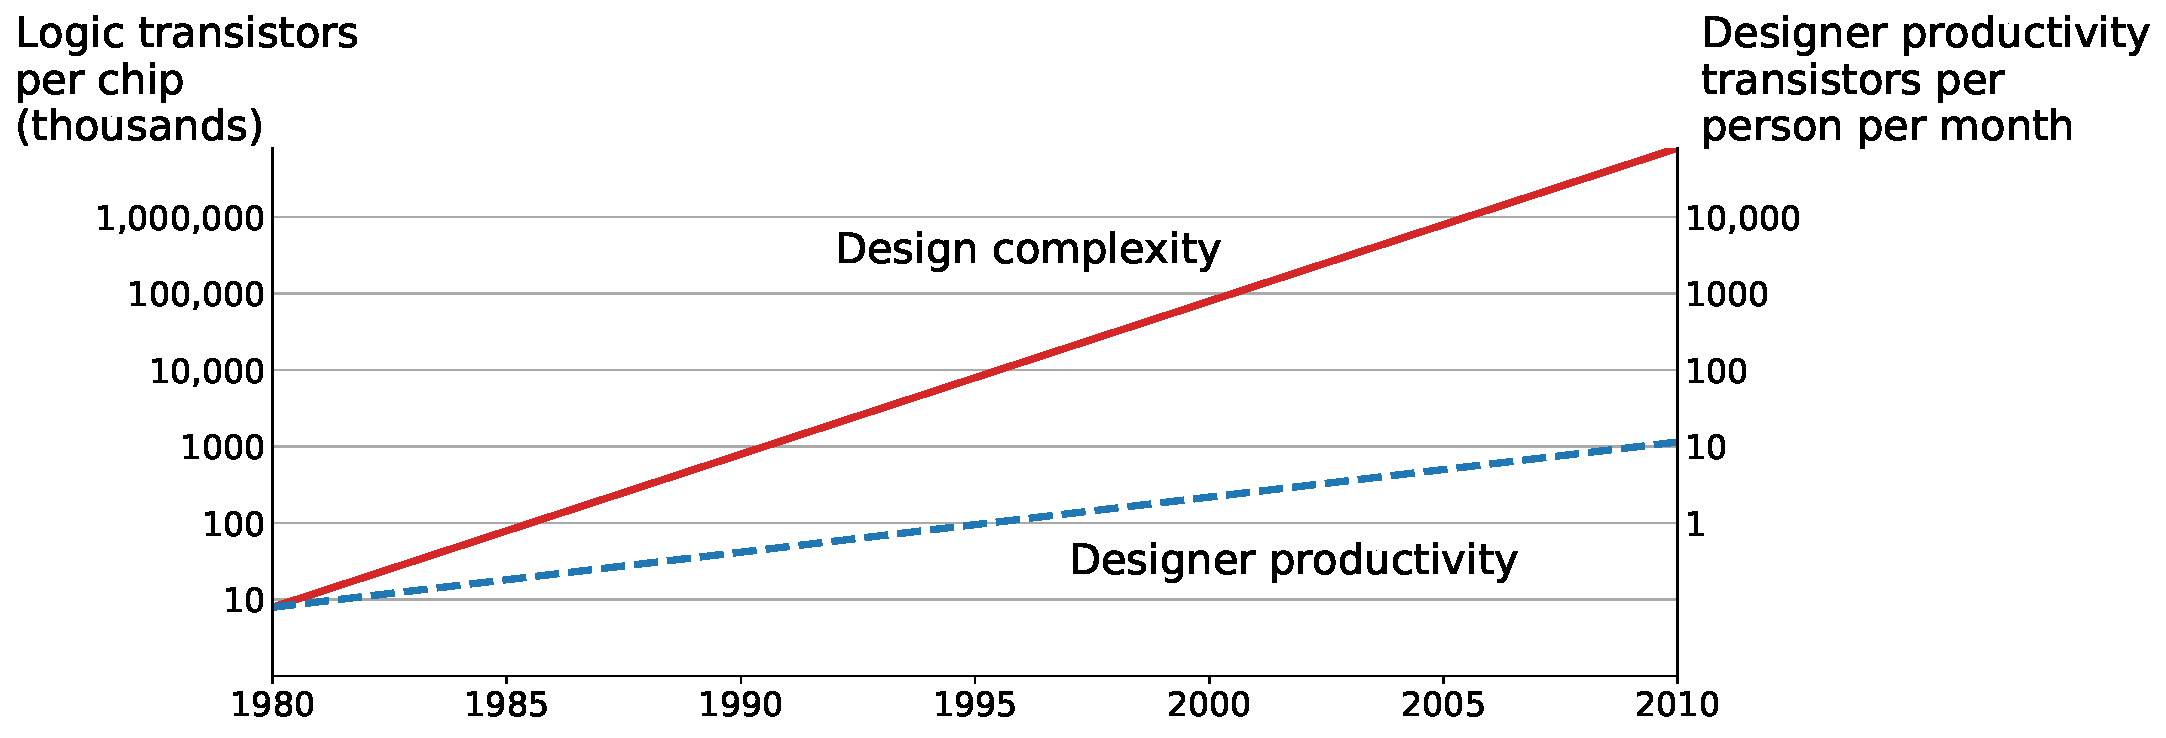
\includegraphics[width=\textwidth]{plots/productivity.pdf}
    \caption{Design complexity and designer productivity trends}
    \label{fig:productivity}
\end{figure}

One of the commonly-accepted solutions for closing the productivity gap as proposed by semiconductor roadmaps is to \emph{raise the level of abstraction in the design process.}
In order to achieve the acceptable productivity gains and to bridge the semantic gap between higher abstraction levels and low-level implementations, the goal now is to \emph{automate} the system-design process as much as possible.
However, to make automation possible we need to have: 1)A well-defined system abstraction level, well-known components of particular abstraction level and having a clear semantics for system-design languages.
The code, however, can be generated in a specific target language such as C>
In order to understand system-level possibilities more fully, we first explain the different abstraction levels involved in system design.

%!TEX root = ../main.tex

% NOTES:
%   * There is a shift to accelerator design
%   * CPUs are inefficient
%   * Fixed accelerators are hard to program
%   * Alternative is FPGA/CGRA
%   * There are challenges with programming FPGA/CGRA
%   * HLS is one solution

%


\section{Abstraction Levels}

The growing capabilities of silicon technology over the previous decades has forced design methodologies and tools to move to higher levels of abstraction
In order to explain the relationship between different design methodologies on
different abstraction levels, we will use the Y-Chart~\cite{walker_1985_y_model} to explain differences between different design tools and different design methodologies in which these tools were used.

\begin{figure}[h]
    \centering
    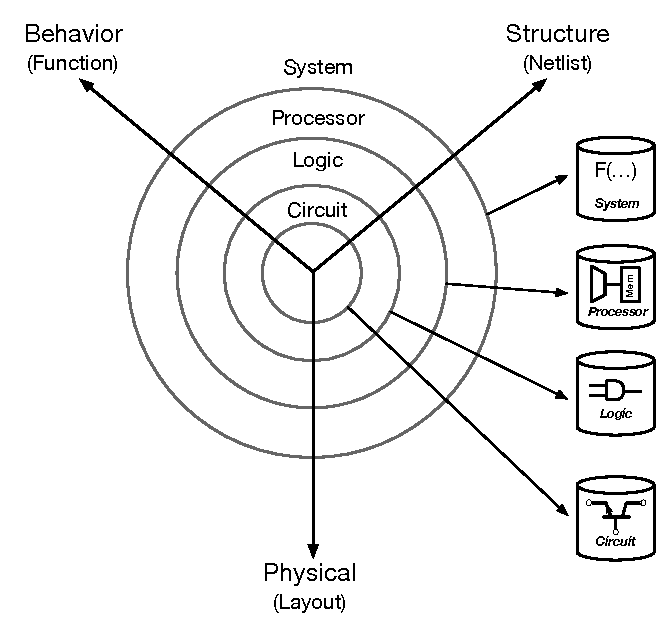
\includegraphics[width=0.5\textwidth]{figures/Introduction/Y-Chart.pdf}
    \caption{Y-Chart}
    \label{fig:y-chart}
\end{figure}

Y-Chart divides design representation into three domains:1)Behavioral, it can also called functionality and specification, 2)Structural, also called netlist or a block diagram and 3)Physical, usually called layout or board design. Behavior represents a design as a black-box but it describes the output base on inputs over time. What behavior representation doesn't specify is how the black-box is structured or how to build the black-box. This is the task of structural representation. In this specification, black-box is represented as a set of components and connections. While, it's possible to drive the behavior of black-box from its components and its connections but understanding the behavior can be very difficult since it is obscured by the details of each component and connection.
Eventually, physical design describe different dimension of each component.

The Y-chart also defines multiple level of abstractions for a design by drawing concentric circles on the Y. Typically, four levels are used: system, processor, logic and circuit levels.
The name of each abstraction level is derived from the types of the components generated on that abstraction level.
For instance, on the processor level, we generate standard and custom processors, or special-hardware components such as memory controllers, arbiters, brides and various interface components. At the higher level, system level, we design standard or embedded systems consisting of processors, memories, buses, and other processor components.

Let's look at binary counter as an example. In this example at the algorithmic-level, we only know that at every cycle the input value will be increased by one and the output in the next cycle would be the input plus one.
At the next lower level, we understand that to carry out this function some sort of register is needed to hold the value of the counter.
We can state this idea using a register transfer statement such as $AC \leftarrow AC + 1$.
On the structural side, the register consists of gates and flip-flops, which themselves consist of transistors.

On each abstraction level, we need a library of components to be used in building \emph{the structure} for a given \emph{behavior}.
This process of converting the given behavior into a structure for a given haviour is called \textbf{synthesis}.
Once a structure is defined and verified, we can proceed to the next lower abstraction level by further synthesizing each of the components in the structure.
On the other hand, if each component in the library is given with its structure and
the physical implementation, we can proceed with physical design.
Thus each component in the library may have up to three different models representing
three different axes in the Y-Chart: behavior or function; structure, which
contains the components from the lower level of abstraction; and the physical.

In the rest of this chapter we focus on the first two level of abstractions, \textit{Processr} and \textit{System}.
Fortunately, all three models for each component are not typically needed most of the time.
Most of the methodologies presently in use perform design or synthesis on the system and processor levels, where every system component except standard processors and memories is synthesized to the logic level, before the physical design is performed on the logic level.
Therefore, for the top three abstraction levels, we only need a functional model of each component with estimates of the key metrics such as performance, delay, power, cost, size, reliability, testability, etc.
Once the design is represented in terms of logic gates and flip-flops, we can use standard cells for each logic component and perform layout placement and routing.
On the other hand, some components on the processor-and-system levels may be obtained as IPs and not synthesized.
Therefore, their structure and physical design are known, at least partially, on the level higher than logic level.
In that case, the physical design then may contain components of different sizes and from different levels of abstraction.

We first explain behavioral model and structural model of each level of abstraction. And then we explain the procedure or moving from behavioral domain to procedural domain.


\section{Behavioral Model}
\label{sec:processor_level_behavioral_model}

On the processor level, we define and design computational components or processing elements (PEs).
Each PE can be a dedicated or custom component that computes some specific functions, or it can be a general or standard PE that can compute any function specified in some standard programming language.
The functionality or behavior of each PE can be specified in several different ways.

In the basic implementation of PEs, their functionality can be specified with mathematical expressions or formulas.
But there is no limitation on what the functionaly of a PE can be.
Therefore, we can expand the functionality of a PE and specify it with an algorithm in some \textit{programming language}.
If we want to go beyond a mathematical expression, we solution is to use Finite State Machines (FSMs).
A FSM is defined with a set of states and a set of transitions from state to state, which are taken when some input variables reach the required value. Furthermore, each FSM generates some val- ues for output variables in each state or during each transition. A FSM model can be made clock-accurate if each state is considered to take one clock cycle. In general, a FSM model is useful for computations requiring several hundred states at most.

This FSM model use standard integer or floating-point variables and computing their values in each state or during each transition by a set of arithmetic expressions or programming statements.
For example, Figure~\ref{fig:fsm_model} shows a FSM with three states, S1, S2, and S3, and with arcs representing state changes under different inputs.
Each state executes a computation represented by one or more arithmetic expressions or programming statements.
For example, in state S1, the FSM in Figure~\ref{fig:fsm_model} computes two functions, $x = |a|$ and $y = |b|$, and in state S3 it computes the function $z = max (x, y)$.
A FSM model is usually not clock-accurate since computation in each state may take more than one clock cycle.
Therefore, using FSM model to represent computation expressed by programming languages like C is not adequet.

\begin{figure}[h]
    \centering
    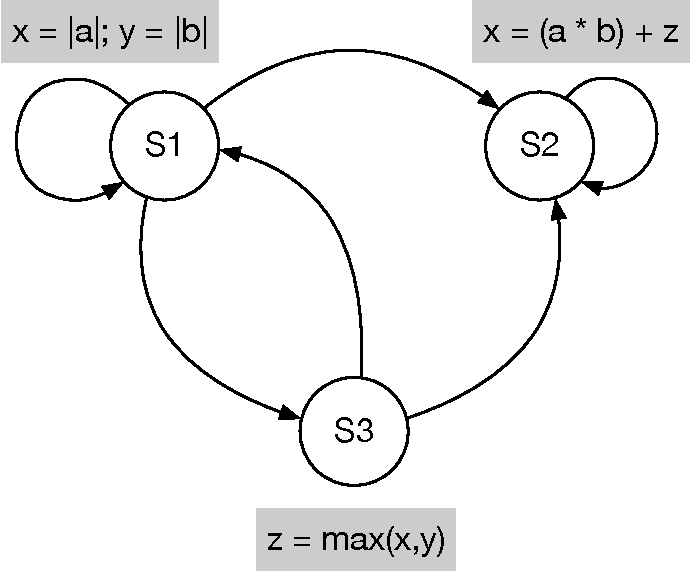
\includegraphics[width=0.4\textwidth]{figures/Introduction/FSM.pdf}
    \caption{FSM model}
    \label{fig:fsm_model}
\end{figure}


In general, programming languages consist of \code{if} statements, loops, and expressions.
An \code{if} statement has two parts, then and else, in which then is executed \code{if} the conditional expression given in the \code{if} statement is true, otherwise the else part is executed.
In each of the then or else parts, the \code{if} statement computes \emph{a set of expressions called a Basic Block (BB)}.
The \code{if} statement can also be used in the loop construct to represent loop iterations, which are executed as long as the condition in the \code{if} statement is true.
Therefore, any programming-language code can be represented by a Control-Data Flow Graph (CDFG) consisting of \code{if} diamonds, which represent \code{if} conditions, and BB blocks, which represent computation [151].
Figure~\ref{fig:dcfg_model} shows such a CDFG, this one representing a loop with an \code{if} statement inside the loop iteration.
In each iteration, the loop construct executes BB1 and BB2 or BB3 depending on the value of \code{if} statement.
At the end, the loop is exited if all all iterations are executed.

A CDFG shows explicitly the control dependencies between loop statements, if statements, and BBs, as well as the data dependences among operations inside a BB.
It can be converted to a FSM by assigning a state to each BB and one state for the computation of each if conditional.
Note that each state in such a FSM may need several clock cycles to execute its assigned BB or if condition.

\begin{figure}[h]
    \centering
    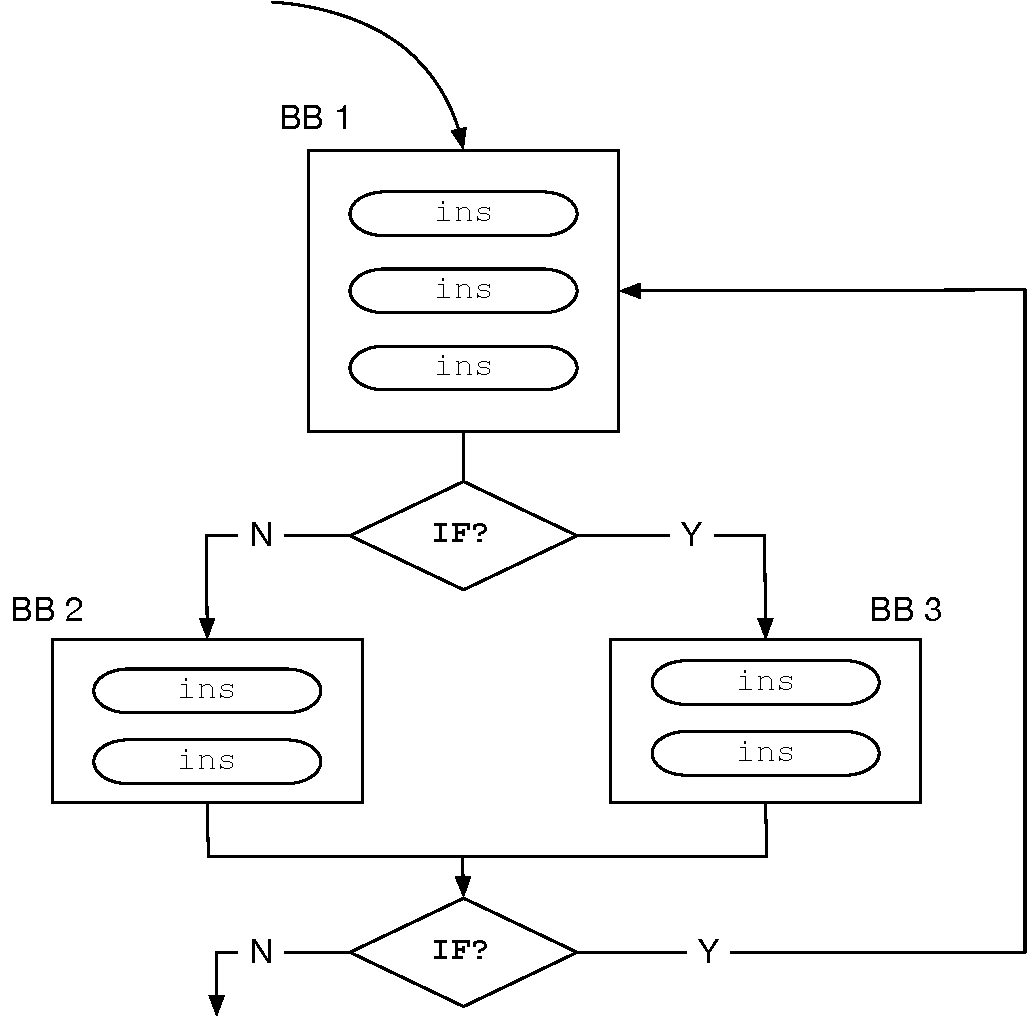
\includegraphics[width=0.55\textwidth]{figures/Introduction/CFG.pdf}
    \caption{FSM model}
    \label{fig:dcfg_model}
\end{figure}

\section{Structural Model}

A processor’s behavioral model, whether defined by a program in C, CDFG, FSM, or by an IS, can be implemented with a set of register-transfer components; such a structural model usually consists of a controller and a datapath like general purpose processors.
A datapath consists of a set of storage elements (such as registers, register files, and memories), a set of functional units (such as ALUs, multipliers, shifters, and other custom functional units), and a set of busses.
All of these register-transfer components may be allocated in different quantities and types and connected arbitrarily through busses or a network-on-chip (NOC).
Each component may take one or more clock cycles to execute, each component may be pipelined, and each component may have input or output latches or registers.
In addition, the entire datapath can be pipelined in several stages in addition to components being pipelined by themselves.
The choice of components and datapath structure depends on the metrics to be optimized for particular implementation.

The controller defines the state of the processor clock cycle per clock cycle and issues the control signals for the datapath accordingly.
The structure of the controller and its implementation depends on whether the processor is a standard processor (such as Xeon, ARM, or a DSP) or a custom-design processor or Intellectual Property (IP) function specifically synthesized for a particular application and platform.
For instance, in the case of a standard processor, the controller is programmable with a program counter (PC), and an address generator (AG) that defines the next address to be loaded into the PC.
In the case of specific custom processors, the controller can be implemented with programmability concepts typical of standard processors, and control signal generation of IP implementations like CGRAs.

\begin{figure}[h]
    \centering
    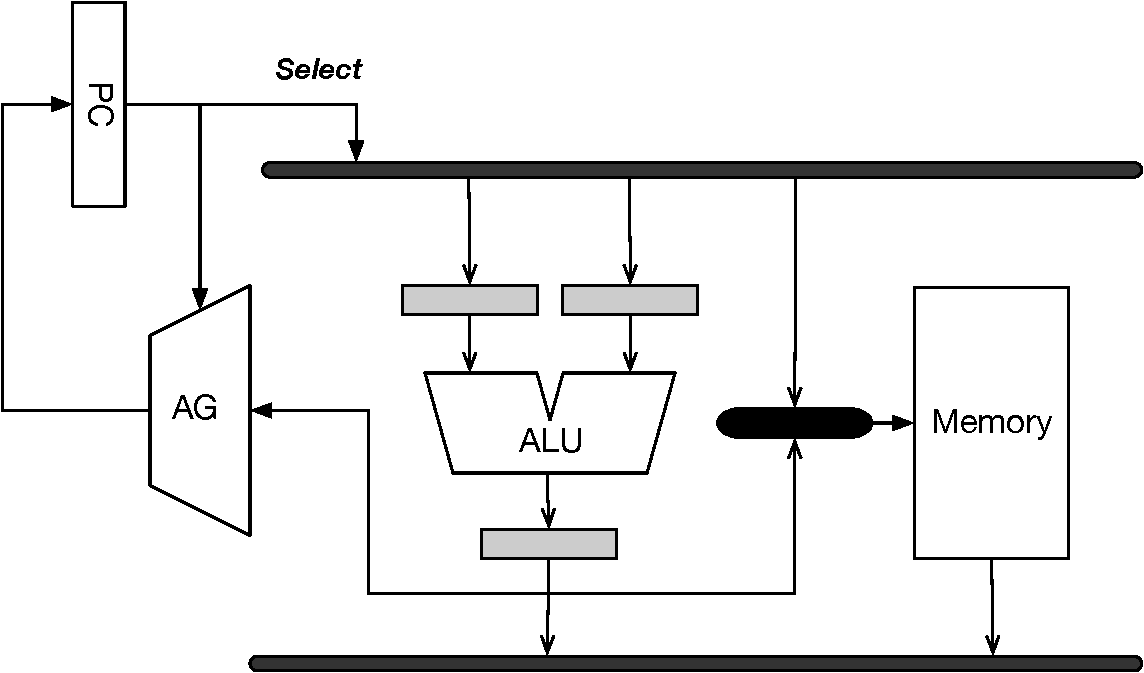
\includegraphics[width=0.6\textwidth]{figures/Introduction/Processor_Structure.pdf}
    \caption{Processor structure model}
    \label{fig:proc_structure}
\end{figure}



\section{Processor-Level Synthesis}

Synthesis of standard processors starts with the instruction set (IS) of the processor.
In order to achieve the highest processor performance this process is done manually since standard processors try to achieve the highest performance and minimal power consumption at minimal cost.
The second reason for synthesizing processors manually is to minimize the design size and therefore fabrication cost for high-volume production.
In contrast, the design or synthesis of a custom processor or a custom IP starts with the C code of an algorithm, which is usually converted to the corresponding CDFG or FSMD model before synthesis and ends up with a custom processor containing the number and type of components connected as required by the given behavioral model.
This generation is usually called high-level synthesis or register-transfer synthesis or occasionally just processor synthesis.
Selecting components and the structure of a PE and \emph{defining register-transfer operations performed in each clock cycle is the task of processor-level synthesis.}

\begin{figure}[h]
    \centering
    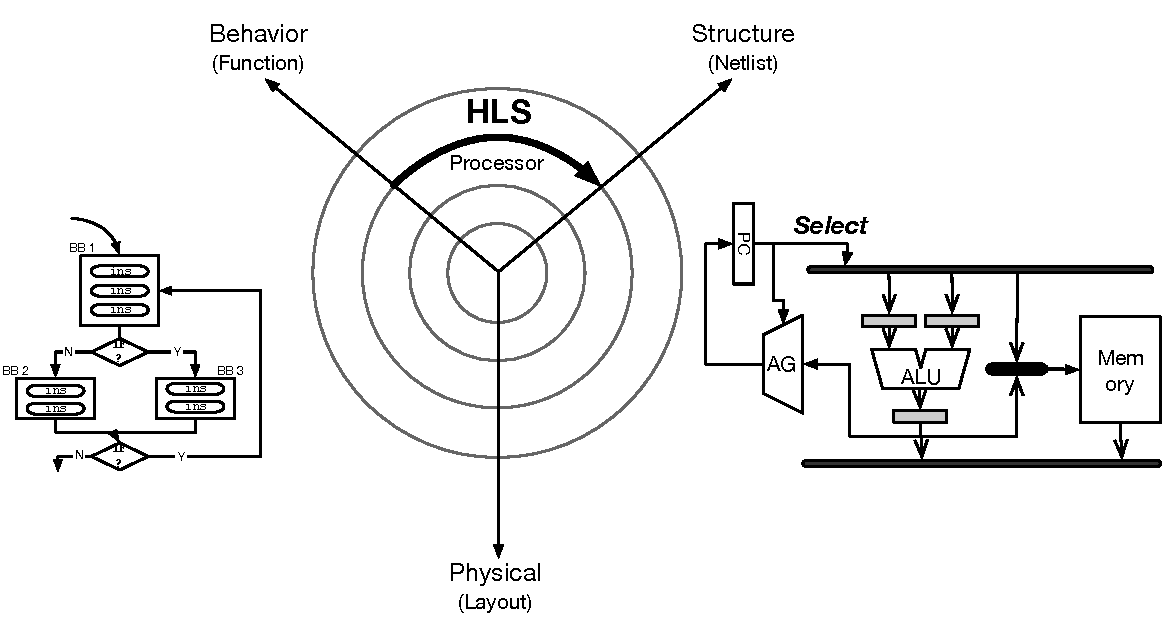
\includegraphics[width=0.9\textwidth]{figures/Introduction/processor-synthesis.pdf}
    \caption{High-Level Synthesis (HLS)}
    \label{fig:proc_synthesis}
\end{figure}


\section{System-Level Synthesis}

Processor-level behavioral models such as the CDFG can be used for specifying a single processor, but will not suffice for describing a complete system that consist of many communicating processors.
A system-level model must represent multiple processes running in parallel in SW and HW.
The easiest way to do this is to use a model which retains the concept of states and transitions as in a FSM but which extends the computation in each state to include processes or procedures written in a programming language such as C/C++.
Furthermore, in order to represent a many-processor platform working in parallel or in pipelined mode, we must introduce concurrency and pipelining.
Since processes in a system run concurrently, we need a synchronization mechanism for data exchange, such as the concept of a channel, to encapsulate data communication.
Also, we need a model which supports hierarchy, so as to allow designers to write complex system specifications without difficulty.
Figure~\ref{fig:task_graph} illustrates such a model of hierarchical sequential-parallel processes, which is
usually called a Process State Machine (PSM).
This particular PSM is a system-level behavior or system specification, consisting of processes P1 to P5.
The
system starts with P1, which in turn triggers process P2 if condition d is true, or
another process consisting of P3, P4, and P5 if condition d is not true. P3 and
P4 run sequentially and in parallel with P5, as indicated by the vertical dashed
line. When either P2 is finished or the sequential-parallel composition of P3,
P4, and P5 is finished, the execution ends.

\begin{figure}[h]
    \centering
    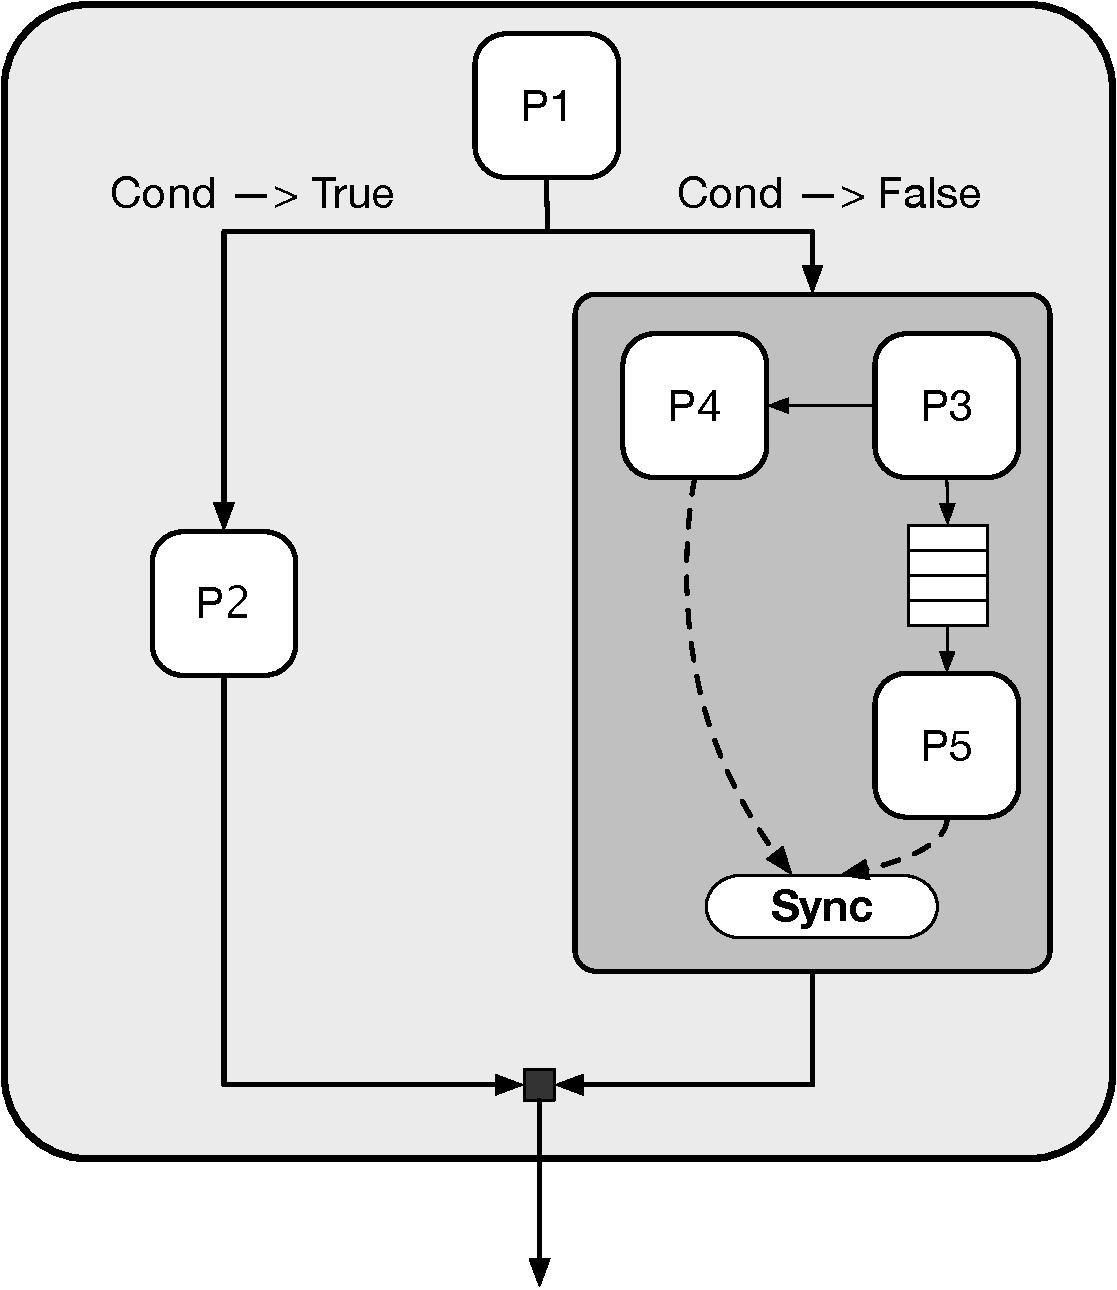
\includegraphics[width=0.4\textwidth]{figures/Introduction/Task_Graph.pdf}
    \caption{System behavioral model}
    \label{fig:task_graph}
\end{figure}


In the synthesis part we need to answer question like what is the memory model. How is the memory shared across different processes.



\subsection{Missing Semantics}
\label{sec:missing_semantics}

A big challenge in \emph{synthesising} is missing semantics. In many cases there are many different representation and design for a same behavioral model. But which model fits better in our design. 
As an example of this problem, we can look in ~\ref{fig:missing_semantics} at a simple case statement available in any hardware or system modeling language.
This type of case statement can be used to model a FSM in which every case such as X1,X2, ..., represents a state in which all its next states are de ned.
This type of case statement can also be used to model a look-up table, in which every case X1, X2, ..., indicates a location in the memory that contains a value in the table.
Therefore,  we can use the same case statement with the same variables and format to describe two completely different components.
Unfortunately, FSMs and look-up tables require completely different implementations:  a FSM can be implemented with a controller or with logic gates, while a look-up table is usually implemented with some kind of memory.
It is also possible to implement a FSM with a memory or a table using logic gates.
However, this would not bea very ef cient implementation, and it would not be acceptable to any designer.
So a model which uses case statements to model FSMs and tables is good for simulation but not for implementation because neither a designer nor a synthesis tool can determine which type of structure was described by the case statement.
The lesson is that contemporary modeling languages allow modelers to de-scribe the design in many different ways and to use the same description for different designs details. But for automatic refinement, synthesis, and veri cation, we need clean and unambiguous semantic which uniquely represents all the system concepts in a given model.  Such a clean semantic is missing from most of the simulation-oriented  languages.
In order to have well defined semantics, we need to introduce some form of formalism to models and modeling languages.


\begin{figure}[h]
    \centering
    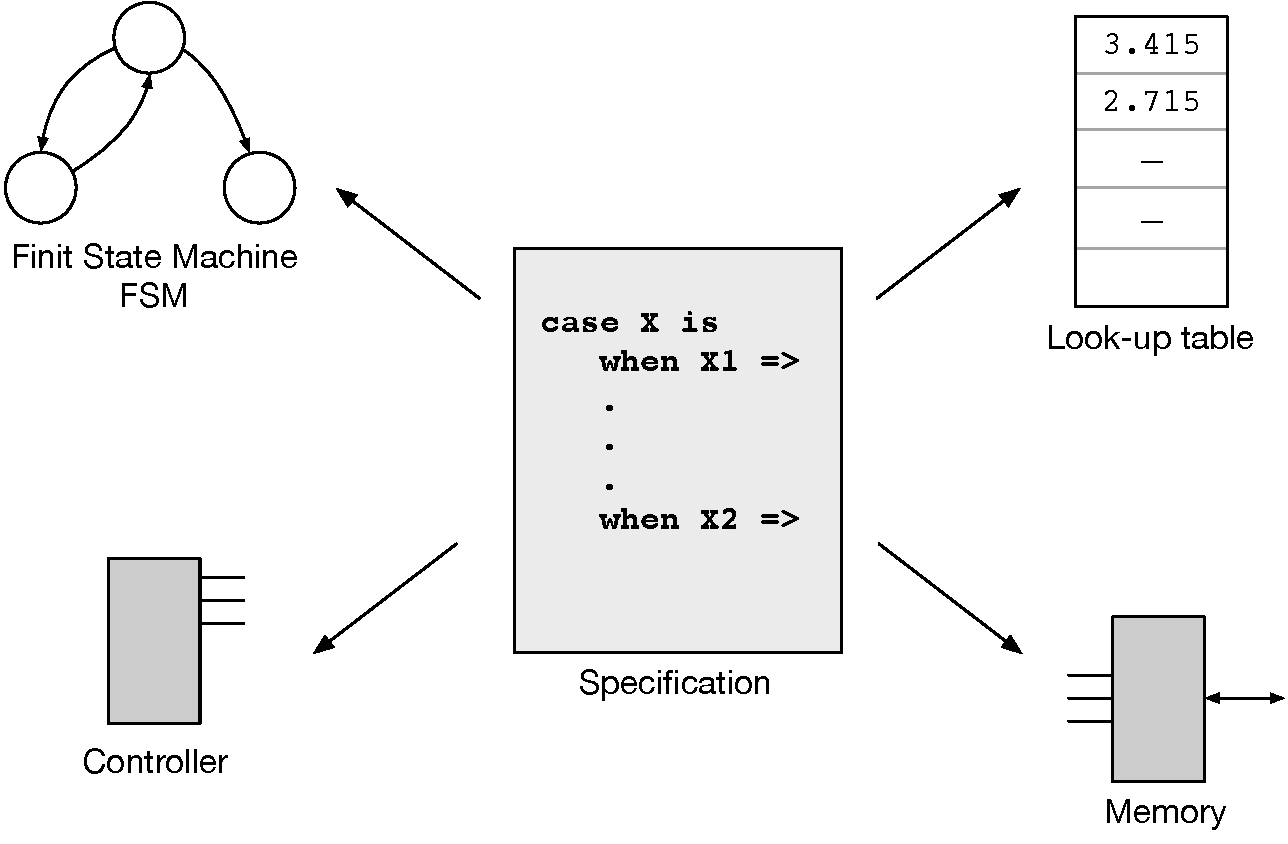
\includegraphics[width=0.7\textwidth]{figures/Introduction/Missing_Semantics.pdf}
    \caption{Missing Semantics}
    \label{fig:missing_semantics}
\end{figure}


\section{Hardware Design Methodologies}

\paragraph{Method1:} Describe-and-Synthesize methodology (late 1980s to late 1990s).
The 1980s brought us tools for logic synthesis which have significantly altered design flow, since the behavior and structure of a design were both captured on the logic level.
Designers specified first what they wanted in Boolean equations or FSM descriptions, and then the synthesis tools generated the implementation in terms of a logic-level netlists.
In this methodology therefore, the behavior or function comes first, and the structure or implementation comes afterwards.
Moreover, both of these descriptions are simulatable, which is an marked improvement over Capture-and-Simulate methodology, because it permits much more efficient verification; it makes it possible to verify the descriptions’ equivalence since both descriptions can in principle be reduced to a canonical form.
However, today’s designs are too large for this kind of equivalence checking.
By the late 1990s, the logic level had been abstracted to the Register-Transfer Level (RTL) with the introduction of cycle-accurate modeling and synthesis.
Therefore, we now have two abstraction levels (RTL and logic levels) and two different models on each level (behavioral and structural).
However, the system gap still persists because there was not relation between RTL and higher system level.

\paragraph{Method2:}  The 1980s brought us tools for logic synthesis which have significantly altered design flow, since the behavior and structure of a design were both captured on the logic level.
Designers specified first what they wanted in Boolean equations or FSM descriptions, and then the synthesis tools generated the implementation in terms of a logic-level netlists.
In this methodology therefore, the behavior or function comes first, and the structure or implementation comes afterwards.
Moreover, both of these descriptions are simulatable, which is an marked improvement over Capture-and-Simulate methodology, because it permits much more efficient verification; it makes it possible to verify the descriptions’ equivalence since both descriptions can in principle be reduced to a canonical form.
However, today’s designs are too large for this kind of equivalence checking.

By the late 1990s, the logic level had been abstracted to the Register-Transfer Level (RTL) with the introduction of cycle-accurate modeling and synthesis.
Therefore, we now have two abstraction levels (RTL and logic levels) and two different models on each level (behavioral and structural).
However, the system gap still persists because there was not relation between RTL and higher system level.


\paragraph{Methode3:}
Specify, Explore-and-Refine methodology (early 2000s to present).
In order to close this gap, we must increase the level of abstraction from the RTL to the system level (SL) and to introduce a methodology that includes both SW and HW.
On the SL, we can start with an executable specification that represents the system behavior; we can then extend the system-level methodology to include several models with different details
that correspond to different design decisions. Each model is used to prove some system property: functionality, application algorithms, connectivity, communication, synchronization, coherence, routing, performance, or some design metric such as performance, power, and so on.
So we must deal with several models in order to verify the impact of design decisions on every metric starting from an executable specification down to the RTL and further to the physical design.
We can consider each model as a specification for the next level model, in which more implementation detail is added after more design decisions are made.
We can label this a Specify-Explore-Refine (SER) methodology [63, 100], in that it consists of a sequence of models in which each model is a refinement of the previous.
Thus SER methodology follows the natural design process in which designers specify the intent first, then explore possibilities, and finally refine the model according to their decisions.
SER flow can therefore be viewed as several iterations of the basic Describe-and-Synthesize methodology.

In order to explain about SER model first we overview the status of methodologies presently in use, their shortcomings, and how to upgrade them to the system level.


%!TEX root = ../main.tex

% Notes 

\chapter{Related Works}

\section{Hardware Definition Languages (HDL)}

Hardware description languages like Verilog and VHDL are designed for arbitrary circuit description.
Initially, these languages are developed as hardware simulation languages, and were only later adopted as a basis for hardware design.
While HDL language syntaxes resemble software languages but their concepts are inherently different from software languages.
Software programs are designed to describe an algorithm for processors.
They have sequential semantics and correctness of the program is defined as executing instructions in the order the instructions are written.
Data movement is implicit between instructions and there is a explicit defined memory model.
In contrast, HLD languages are designed to specify circuit designs.
Hardware inherently is concurrent and each statement in HDL language is concurrent with other statements.
All the dependencies need to be explicit either in the form of wire or register.
There is no pre-defined memory model. Memory model needs to be explicitly defined and handled in the design.
Because the semantics of these languages are based around simulation, synthesizable designs must be inferred from a subset of the language, complicating tool development and designer education.
HDL languages do not contain a clear semantic just like software languages, as a result, HLD languages can result in ambiguities that make automated synthesis and verification impossible, due to the unclear semantics involved.
Moreover, for any design, in order to achieve maximum generality, they require users to explicitly manage timing, control signals, and local memories.

A big limitation of HDL languages is that these languages lack the powerful abstraction and facilities that are common in modern software languages, which leads to low designer productivity.
For instance, reusability is one of such powerful facilities that HDL languages inherently are aboard to reuse hardware modules~\cite{shacham_rethinking_2010}.
Recent extensions such as SystemVerilog~\cite{systemverilog} improved the type system and parameterized generate facilities but still lack many powerful programming language features.
The key benefit of reusing hardware components is that every time a chip is built, we inherently evaluate different design decisions, either implicitly using microarchitectural and domain knowledge, or explicitly through custom evaluation tools.
Rather than building a custom chip, designers create a template, or a chip generator, that can generate the specialized chip.
For instance, Tensilica applied the same idea to create customized processors~\cite{tensillica}.


Constructing efficient hardware designs requires extensive design-space exploration of alternative system microarchitectures. 
This is another limitation of HLD languages, traditional HLDs have limited support for auto generating modules and are ill-suited to producing and composing the highly parameterized module generators required to support through design-space exploration.

The first step to synthesis behavioral description model to structural structural model is having more powerful hardware languages that can support such important features like enabling hardware reusability, templatizing and hardware modules. In addition, it let's the compiler to efficiently search the design-space for alternative system designs. In the following we look at some of the works to improve and add such features to traditional HLD languages and talk about pros and cons of each approach.

\subsection{BlueSpec}

One alternative proposal to improve productivity of HLD languages is beginning from a domain-specific application programming language and then generate hardware blocks. 
Bluespec~\cite{bluespec} is an example of such languages.
Bluespec Compiler (BSC) is a tool that uses BluespecSystem  Verilog  (BSV)  as  the  design  language.
BSV is a high-level functional HDL based on Verilog and inspired by Haskell, where  modules are implemented as a set of rules using  Verilog  syntax.
In this language, the concurrent behavior of a system is expressed as a collection of rewrite rules.
The rules are called guarded atomic actions and express behavior in the form of concurrently cooperating finite state machines (FSMs).
Rules are predicated with a condition. They give the impression of freezing the rest of the system when a given rule's action is carried out after the rule's predicate is true.
There is an implicit parallelism in this specification, because it is possible for multiple rules to be activated and executed in parallel.
The compiler automatically schedules the rules such that they are either conflict-free or combined sequentially to preserve the promised atomicity semantic.
Please find a counter example, implemented in Bluespec, in  Appendix.

While these can provide great designer productivity when the task in hand matches the pattern encoded in the application programming model, they are a poor match for tasks outside their domain.
For example, the design of a programmable microprocessor is not well described in a stream
programming model, and guarded atomic actions are not a natural way to express a high-level DSP algorithm.
Furthermore, in general it is difficult to derive an efficient microarchitecture from a higher-level computation model, especially if the goal is a programmable engine to run many applications, where the human designer would prefer to write a generator to explore this design space in detail.


\section{Hardware Constructor Languages (HCL)}
\subsection{Genesis2}
Genesis2~\cite{genesis2} was one of the first attempts to work around mentioned limitations, specially reusability. Genesis2 uses Perl language as a macro processing language to provide more flexible parameterization and elaboration of underlying hardware blocks in SystemVerilog. Listing~\ref{listing:genesis2} shows an example of \textit{Genesis2's code}.
In this example, perl is using ceil library from POSIX library to set the values for $\$num\_add\_bits$.

\begin{listing}[ht]
    \begin{minted}
        [xleftmargin=20pt,
        autogobble,
        linenos] 
        {Verilog}
//; # More Perl Libraries
//; use POSIX (ceil);
//; my $reg_list = $self->define_param(REG_LIST => 
//; [	
//;     {name => 'regA', width => 5, default => 17, IEO => 'ie'},
//;     {name => 'regB', width => 15, IEO => 'ieo'},
//;     {name => 'regC', width => 32, IEO => 'ieo'},
//; ]);
//; my $num_regs = scalar(@{$reg_list});
//; my $num_addr_bits = ceil(log($num_regs)/log(2));

// Verilog code for the module
module 'mname()' (
    input                               Clk,
    input                               Reset,
    input ['$num_addr_bits-1':0]        Addr,
    ...
    );

endmodule // 'mname()'
    \end{minted}
    \caption[Caption for LOF]%
    {Genesis2 code example, combining SystemVerilog and Perl~\cite{genesis2}}
    \label{listing:genesis2}
\end{listing}


These approaches allow familiar and powerful languages like Verilog to be macro languages for hardware netlists, but effectively require leaf components of the design to be described in the underlying HDL.
This combined approach is cumbersome, combining the poor abstraction facilities of the underlying HDL with a completely different high-level programming model that does not understand hardware types and semantics.

\subsection{Chisel and FIRRTL}

Chisel~\cite{chisel} is another successful, modern, generalize HCL which is a domain specific language (DSL) for describing hardware circuits embedded in Scala.
Chisel provides modern programming language features such as meta-programming and object oriented concept coupled with library availability for accurately specifying low-level hardware blocks, but which can be readily extended to capture many useful high-level hardware design patterns.
To see how Chisel could improved the limitations of traditional HDL languages, we try to answer the following question:
\emph{What benefits does Chisel offer over classic Hardware Description Langues?\footnote{\url{https://github.com/freechipsproject/chisel3}}}
There are two main angles to this question: 1)Chisel improved productivity through new language features, like object oriented programming, functional programming and availability of reusable libraries. 2)Improved specialization due to the hardware-compiler structure. We elaborate more on these two angles in the continue.

Chisel by itself do not provide any new hardware abstractions. However, host language features, Scala, allow designs to be more parameterizable and modular~\cite{izraelevitz_2017_firrtl_reusability}.
For instance,  someone can write a recursive Scala function to construct an adder-reduction tree, parameterized on bit-width.
Unlike the explicitly unrolled version necessary in Verilog, the same generator could be re-used anywhere an adder tree is desired.
Figure~\ref{fig:filter} shows the specified example and the abstract Chisel code.

\begin{figure}[h]
    \centering
    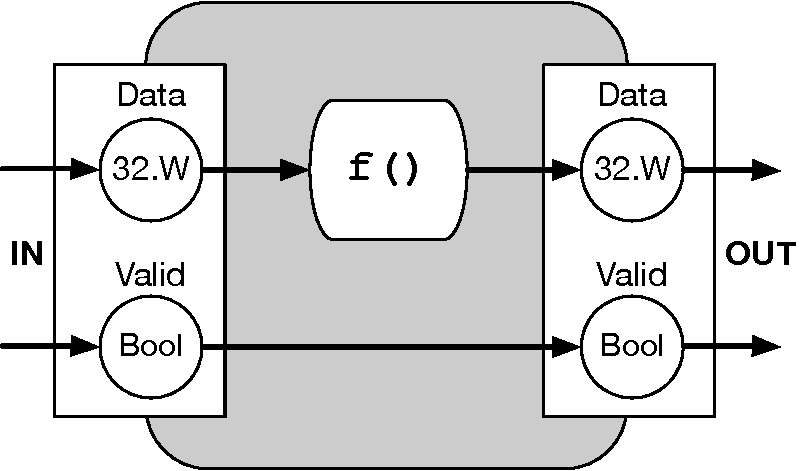
\includegraphics[width=0.45\textwidth]{figures/Introduction/Filter.pdf}
    \caption{Missing Semantics}
    \label{fig:filter}
\end{figure}


\begin{listing}[ht]
    \begin{minted}
        [xleftmargin=20pt,
        autogobble,
        linenos] 
        {Scala}

abstract class Filter[T <: Data](dtype: T) extends Module {
val io  = new Bundle {
val in  = Input(Valid(dtype))
val out = Output(Valid(dtype))
} }

class FunctionFilter[T <: Data](dtype: T, f: T => T) extends Filter(dtype) {
io.out.valid := io.in.valid
io.out.bits := f(io.in)
}

    \end{minted}
    \caption{Chisel abstract function filter}
    \label{listing:chisel_example}
\end{listing}


\begin{listing}[ht]
    \begin{minted}{Scala}

    def clippingFilter[T <: Num](limit: Int, dtype: T) =
        new FunctionFilter(x => min(limit, max(-limit, x)), dtype)

    \end{minted}
    \caption{Chisel abstract function filter}
    \label{listing:chisel_example_f2}
\end{listing}

\begin{listing}[ht]
    \begin{minted}{Scala}

    def shiftingFilter[T <: Num](shift: Int, dtype: T) =
        new FunctionFilter(x => x >> shift, dtype)

    \end{minted}
    \caption{Chisel abstract function filter}
    \label{listing:chisel_example_f3}
\end{listing}


As another example, designer can write a filter module which takes, as a parameter, a higher-order-function that creates the condition checking hardware.
The user of this module then only needs to write the filtering condition, re-using the base filter structure.
There are mature Chisel projects like \emph{Rocket-Chip~\cite{rocket-chip}} and \emph{Diplomacy~\cite{diplomacy}} that can be used as libraries, as examples of Chisel's modularity.
Using these libraries user is being able to \emph{just import a RISC-V microprocessor} in the same way that they \emph{just import a graph library} in software.

The second important advantage of Chisel compare to HDLs is a Hardware Compiler Framework that looks very much like LLVM~\cite{llvm} applied to hardware generation.
The Chisel-to-Verilog process forms part of a multi-stage compiler.
The Chisel front-end compiles Chisel to a circuit intermediate representation called FIRRTL (Flexible Intermediate Representation for RTL)~\cite{firrtl}.
FIRRTL mid-end then optimizes FIRRTL and applies user-custom transformations.
Finally the Verilog back-end emits Verilog based on the optimized FIRRTL.
In this process, FIRRTL represents the standardized elaborated circuit that the Chisel HDL produces.
FIRRTL represents the circuit immediately after Chisel's elaboration but before any circuit simplification.
FIRRTL is designed to resemble the Chisel after all meta-programming has executed. Thus, a user program that makes little use of meta-programming facilities should look almost identical to the generated FIRRT.
In fact, in this architecture Chisel is mostly used for its meta-programming facilities, hence, Chisel front-end can be very light-weight.
Another advantage of such architecture is that other HLD languages, such as Verilog\footnote{Yosys Verilog-to-Firrtl Front-end: \url{https://github.com/cliffordwolf/yosys}} can target FIRRTL and reuse the majority of the compiler toolchain.

While these improvements allow for more powerful meta-programming compared to Verilog \code{generate} statements, users still write programs at a timed circuit level. This is still one of the most important limitation of HCLs to improve the overall \emph{system design productivity}.

\section{Spatial language}
% * Spatial~\cite{david_PLDI_2018_spatial, prabhakar_asplos_2016_parallelpattern}
% * A practice to improve chisel flexibility
% * Higher level of abstraction to chisel
% * Untimed modules
% * Reduction to parallel patterns
Recently, Spatial~\cite{david_PLDI_2018_spatial} is been proposed as a language and compiler for applications specific accelerators.
Spatial focuses on specific type of high-level abstractions required to create a new high level HDL language in which syntax contains memory, control and accelerator-host interface as an individual entities.
Spatial shows these particular constructs within the language are better fit for accelerators specially targeting applications with data locality and data parallelism.
It reduces productivity gap of HDL, structural languages, by increasing the level of abstraction of HDL languages.
In Spatial the design is limited to set of constructs and it allows compiler to optimize the design at the higher-level like optimizing and banking memory modules in the design.
In Spatial, each accelerator is an un-timed module containing  nested loops and customized memory hierarchy. In Listing~\ref{listing:spatial_example} we have shown InnerProduct implementation in Spatial language~\footnote{\url{https://spatial-lang.org/dotprod}}.
In this example, we can see we have two types of memory \code{DRAM} and \code{SRAM}, there is a \code{Reduce} computation pattern and an input mathematic expression.

\begin{listing}[ht]
    \begin{minted}
        [xleftmargin=20pt,
            autogobble,
            linenos] 
        {Scala}

object InnerProduct extends SpatialApp {
    val d1 = DRAM[T](len)
    val d2 = DRAM[T](len)

    Accel {
      // Create local SRAMs
      val s1 = SRAM[T](len)
      val s2 = SRAM[T](len)
      
      // Transfer data
      s1 load d1
      s2 load d2
      
      // Multiply and accumulate
      x := Reduce(Reg[T](0))(len by 1)
      {i => s1(i) * s2(i)}{_+_} 
    }
  }
}

    \end{minted}
    \caption{Chisel abstract function filter}
    \label{listing:spatial_example}
\end{listing}

In fact, Spatial, is a new DSL language on top of Chisel which tries to strike balance between high-level constructs in the language for improving programmer productivity versus low-level syntax for tuning performance. 
For instance, to enable the compiler to be able to reason about the loop structures, Spatial limits the types of control structures into four types: \code{FSMs}, \code{Foreach}, \code{Reduce} and \code{MapReduce}.
Therefore, as long as the designer can express his design in such patterns, compiler can reason about the available parallelism and automatically pipeline the design.
However, in many cases such control structures are note enough to express arbitrary designs.
While Spatial has improved the accelerator design productivity compare to Chisel.
But Spatial is a structural language, hence, the design needs to be implemented in Spatial language.
Therefore, synthesizing arbitrary designs from behavioral description can be very challenging because of the missing semantics existing between behavioral model, software, and structural model, Spatial~\ref{sec:missing_semantics}.
The main goal of Spatial is limiting DSE by defining higher level abstractions on top of Chisel and enabling compiler to only search trough very limited space.

\section{High-Level Synthesis}

High-level synthesis (HLS) techniques have been proposed to improve the productivity of hardware designers by automatically generating the hardware from a high-level description, behavioral description, of an algorithm.
In pure C-to-gates HLS, front-end captures system behavior with a model of computation in a standard language such as C, C++, SystemC as an input.
The language components in this case are in the form of untimed mathematical expressions and nested serial loops, pipeline loops or parallel loops.
In the next step, the compiler statically schedules the input algorithm and applies optimizations such as inner loop pipelining, unrolling, and memory banking and buffering~\cite{chung_micro_2010, lee_1989_new, paulin_1989_force}.
Examples of such HLS tools are LegUp~\cite{canis_2011_legup}, Vivado HLS~\cite{vivadohls}, Intel’s FPGA SDK for OpenCL~\cite{opencl_sdk}, and SDAccel~\cite{sdaccel} allow users to write FPGA designs in C/C++ and OpenCL.

To show an example of such limitation of standard HLS approaches, consider the code in Listing~\ref{listing:static_schedule}.
In this loop there is a control flow decision (if) which depends on the actual data being read from arrays A[] and B[].
The operation which might take place in a specific iteration (s = s + d) introduces a dependency between iterations and delays the next iteration whenever the condition is true.
A typical HLS tool needs to create a static schedule for the loops, which means it needs to take the conservative decisions for synthesizing the loop. The compiler has either two choices, make the loop serial and state machine base or make the loop iterations pipeline, which for pipelining it usually need input directives from the input algorithm.
Figure~\ref{fig:no_pipeline} shows the both possible schedules, serial and pipeline, for \code{if} code when we use HLS tools with statically scheduling approach.


\begin{figure*}[ht]
    \begin{minipage}{0.4\linewidth}
        \begin{minted}
            [xleftmargin=20pt,
            autogobble,
            linenos]
            {C}
float d, s = 0.0;
for(int i=0; i<100; i++){
    d = A[i] - B[i];
    if (d >= 0)
    s += d:
}
    \end{minted}
    \end{minipage}
    \begin{minipage}{0.45\linewidth}
        \begin{minted}
            [xleftmargin=20pt,
            autogobble,
            linenos] 
            {C}
float d, s = 0.0;
#pragma pipeline
for (int i=0; i<100; i++){
    d = A[i] - B[i];
    if (d >= 0)
        s += d:
    }
    \end{minted}
    \end{minipage}
    \caption{Limitations of static scheduling}
    \label{listing:static_schedule}
\end{figure*}


\begin{figure}[!h]
    \begin{minipage}[t]{\linewidth}
        \centering
        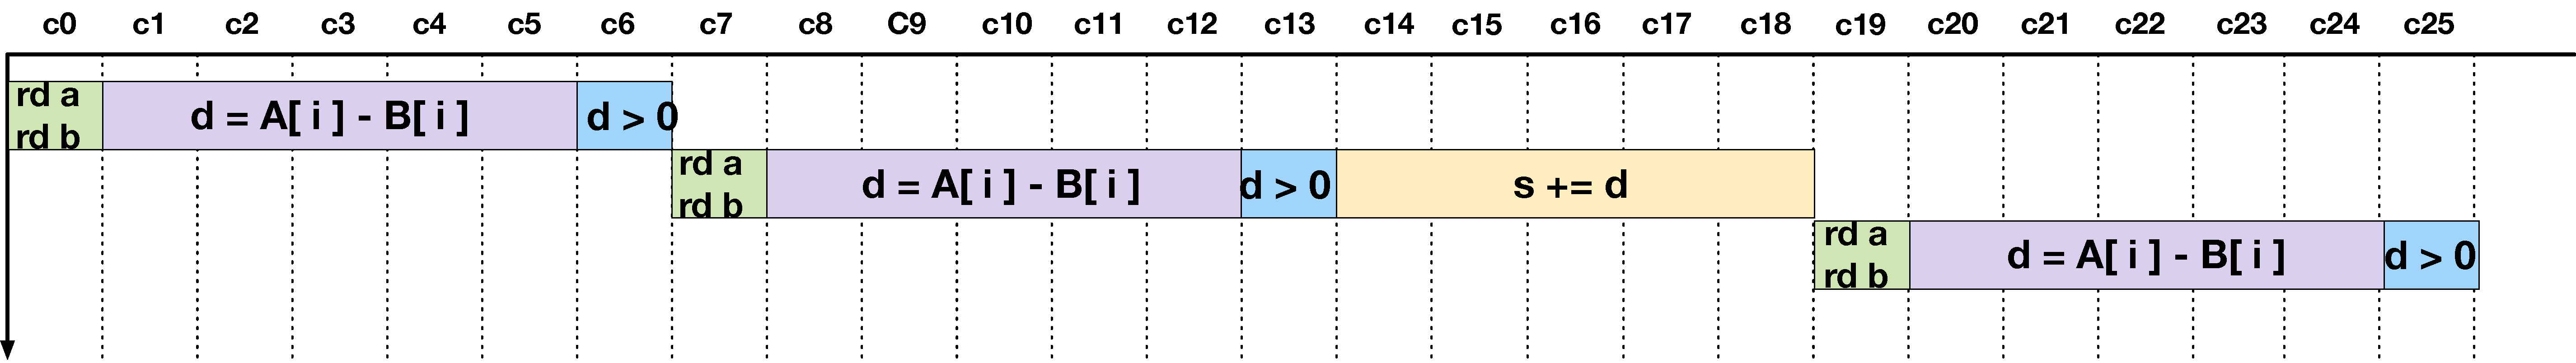
\includegraphics[width=1\textwidth]{figures/Introduction/schedule.pdf}
        \label{fig:no_pipeline}
    \end{minipage}
    \hspace{0.1cm}
    \begin{minipage}[t]{\linewidth} 
        \centering
        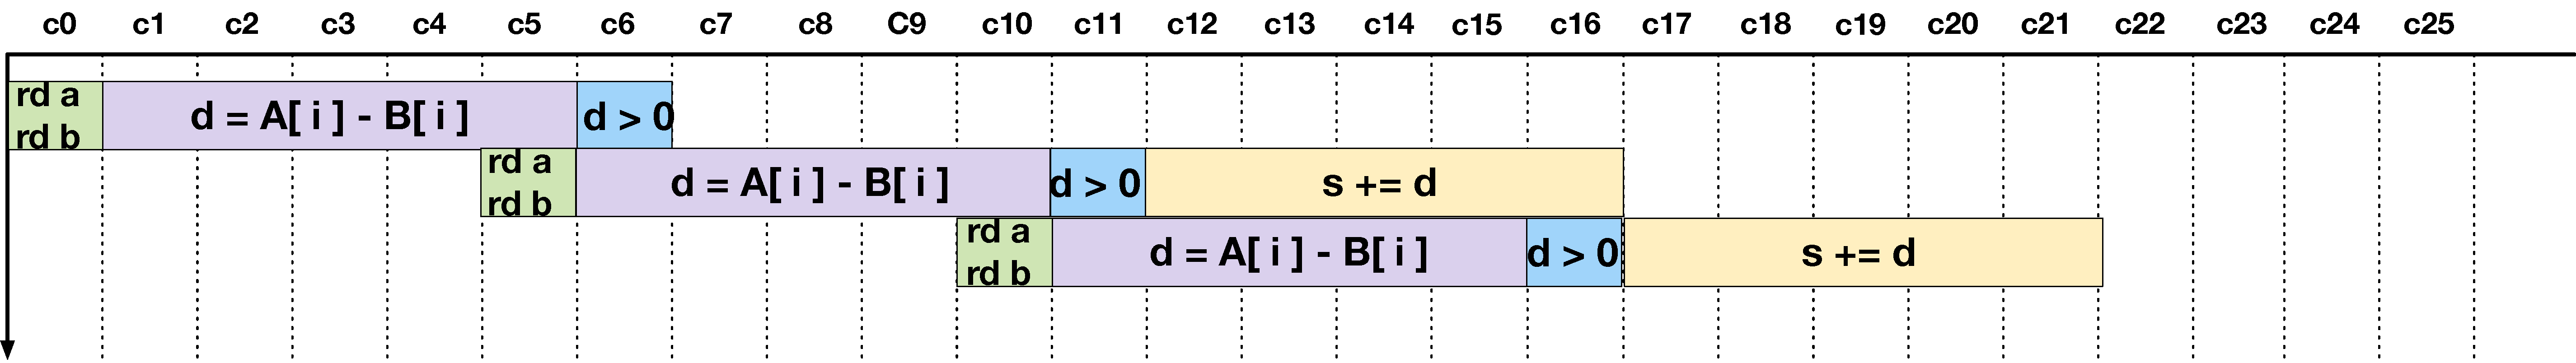
\includegraphics[width=1\textwidth]{figures/Introduction/schedule_pipe.pdf}
        \label{fig:pipeline}
    \end{minipage}        
    \label{fig:schedule}
    \caption{Static Schedule: a)no pipeline, b)pipeline}
\end{figure}  



While traditional HLS tools claim they can support any arbitrary C/C++ programs, however, they input can be always suboptimal and then the major challenge in HLS become how to write a good C/C++ code targeting HLS tool to get the optimal performance~\cite{cong_2018_best}.
One of the most challenging part of implementing FIR filter with HLS is having optimizing input C code for an HLS tools~\cite{cong_2018_best}.
This makes it prohibitive to most software programmers. It is even more challenging when the mainstream algorithm in an application domain is constantly evolving; i.e., an algorithm may have already been obsolete during the development process of its hardware accelerator.
For instance in Figure~\ref{listing:hls_fir_filter} we show the implementation of FIR filter, the same implementation of FIR filter in example~\ref{fig:filter} with Chisel.

In this example, if you look at line number 12, you will see a \code{pragma} that directs the compiler to how to implement the \code{for}.
For instance, in this case, have an efficient implementation of \code{for} loop, the designer needs to know what is the minimum, maximum and average \textit{loop trip counts}.
This information is very low level and it is not trivial specially for software programmers.
The reason is that, these types of \code{pragma}s are actually structural information and since the compiler can not find the optimal structural implementation for a behavioral description, therefore, HLS designers decided to embed this information to the higher level abstraction.

\begin{listing}[ht]
    \begin{minted}
        [xleftmargin=20pt,
        autogobble,
        linenos]
        {C}
    #include "fir.h"

    out_data_t fir_filter(inp_data_t x, coef_t c[N]) {
        static inp_data_t shift_reg[N];
    
        acc_t acc = 0;
        acc_t mult;
        out_data_t y;
    
    Shift_Accum_Loop:
        for (int i = N - 1; i >= 0; i--) {
        #pragma HLS LOOP_TRIPCOUNT min = 1 max = 16 avg = 8
    
        if (i == 0) {
            // acc+=x*c[0];
            shift_reg[0] = x;
        } else {
            shift_reg[i] = shift_reg[i - 1];
            // acc+=shift_reg[i]*c[i];
        }
        mult = shift_reg[i] * c[i];
        acc = acc + mult;
        }
    
        y = (out_data_t)acc;
    
        return y;
    }
    \end{minted}
    \caption{FIR filter for HLS}
    \label{listing:hls_fir_filter}
\end{listing}

Usually such tools adopt polyhedral tools to automate loop pipelining and banking decisions, hence, they reduce the need of adding structural description to the input code.
But such techniques are limited to only affine accesses withing a single loop nest~\cite{wang_2014_theory}, it does not address non-affine cases or cases where accesses to the same memory occur in multiple loop nests.
For instance, Pouchet et al.~\cite{pouchet_2013_polyhedral}  explore combining HLS with polyhedral analysis to optimize input designs for locality and use estimates from HLS tools to drive design space exploration.
While this captures a larger design space than previous work by including tile sizes, this approach is limited to the capabilities of the HLS tools and to benchmarks that have strictly affine data accesses.

Another proposed solution to synthesize control dependencies was synthesizing hyperblocks~\cite{hyperblock}.
Through the use of predication, each hyperblock is transformed into straight-line code and then the computation portion of each hyperblock is implemented speculatively in the form of predicated execution.
CASH~\cite{budiu_cash_2002, budiu_pegasus_2002}, AHRL~\cite{ahrl} and CHiMPS~\cite{chimps} are examples of such technique.
The main disadvantage of this paradigm is the requirement for substantial hardware resources, and it's not a scalable approach. 
In addition, memory layout~\cite{spatial_computation} is another limitation of such approach.

More recent works like Elastic Circuit~\cite{elasticCircuit, elasticFlow}, CGPA~\cite{cgpa} and ~\cite{josipovic_fpga_2018_dynamically} use dynamically schedule circuit to avoid the limitations in inferring loop pipelining.
The idea is to refine from triggering the operators through centralized pre-planned controller but to take scheduling decisions locally in the circuit as it runs.
Therefore, as soon as all the conditions for execution of an operation is satisfied the node has to execute.
Figure~\ref{fig:dynamic_schedule} shows the execution of a dynamically scheduled HLS circuit.
The key reason to a good execution of this loop is that, ideally, a new value of \code{i} should be used to start computing \code{A[i] - B[i]} on every cycle.
While this technique can dynamically provides better schedule compare to other statically scheduled HLS techniques.
But it is clear that, as in the case of processors, taking scheduling decisions dynamically costs resources and time such as the area and delay of the control elements.

\begin{figure}[!h]
    \centering
    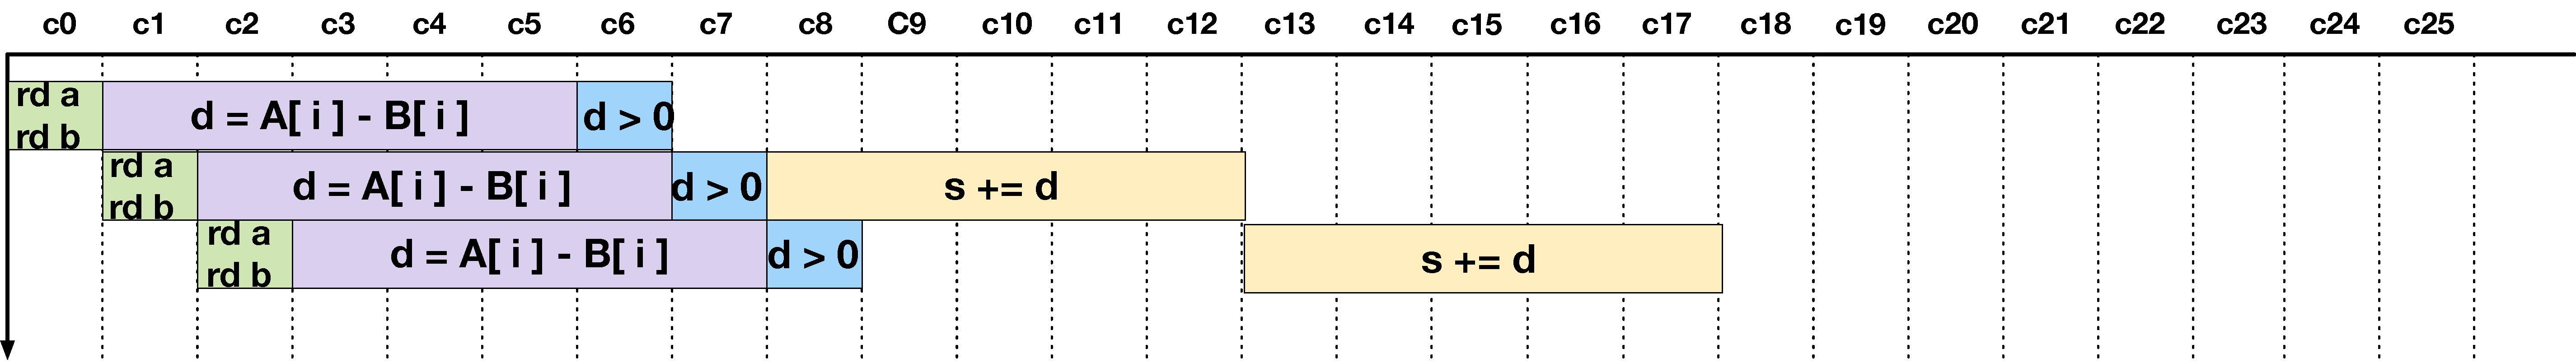
\includegraphics[width=1\textwidth]{figures/Introduction/schedule_dynamic.pdf}
    \label{fig:dynamic_schedule}
    \caption{Dynamically schedule}
\end{figure}  

Overall, all the pure C-to-gates HLS techniques described up to here, rely on capturing parallelism between fine-grain operations of sequential code by constructing the control and dataflow graph (CDFG) of the computation kernels.
Then, they use either scheduling algorithms or dynamic techniques to extract parallelism between the operations that are provably independent in the CDFG.
However, these techniques are less effective in capturing coarse-grain parallelism.
Hence, the Quality of Results (QoR) of these HLS tools are often lower than that of manual design process using low-level hardware-description languages.
Because the highest performance hardware exploits both fine-grain and coarse-grain parallelism.

To extract coarse-grain parallelism, main-stream HLS tools accept parallel programming constructs and/or annotations.
For example, CatapultC~\cite{catapult} and Vivado~\cite{vivado} accepts SystemC~\cite{systemc} processes and modules.
Vivado, also, accepts parallel functions/code-blocks communicating through dataflow channels.
Altera openCL compiler~\cite{opencl_sdk} accepts single instruction multiple thread (SIMT) programming model. 
CMOST~\cite{zhang_DAC_2015_cmost} is a C-to-FPGA framework that uses task-level modeling to exploit multi-level parallelism.
In all these works, the number of input/output iterations and the execution time of each dataflow node for processing the input iteration need to be \emph{static} and known at compile time.
The HLS tools create multiple hardware execution units onto which successive loop iterations are statically scheduled at the hardware construction time.
The down side of this approach is HLS tools must plan for the worst case and allocate resources for all possible iterations regardless of whether they are actually executed, and must handle corner cases.

The alternative approach is task parallelism or \emph{dynamic parallelism}.
The term dynamic parallelism refers to enabling tasks to vary at run-time, both in terms of the type of child task spawned and the number of child tasks spawned.
TAPAS~\cite{margerm_2018_tapas} and ParallelXL~\cite{chen_micro_2018_parallelXL} are the two recent works that addressed the following paradigm.
TAPAS uses a parallel compiler intermediate-representation and includes support for arbitrarily nested parallelism and irregular task parallelism.
And then it builds a parallel accelerator with using a library of hardware components to synthesize spawning and synchronizing tasks, buffering tasks, and inter-task communication.
In contrast, ParallelXL~\cite{chen_micro_2018_parallelXL} adopts continuation passing mechanism to express computation as a dynamic task graph with explicit dependencies.
Using continuation framework as foundation, ParallelXL builds other constructs such as data-parallel loops and for-join patterns on top of it.
The main disadvantage of dynamic parallelism versus static parallelism is trading off performance against hardware utilization.

%%%
Because of regular data access and static nature of signal processing and multi-media workloads, recently there are explicit proposed image processing DSLs.
The narrow domain allows these DSLs to offer high-level specification and more concise abstractions for specifying stencil operations.
These languages usually rely on source-to-source translation and their implementation is a mixture of a DSL language (front-end) and standard HLS tools (back-end).
Recent work on Halide~\cite{halide_pldi_2013} has demonstrated targeting heterogeneous systems by generating intermediate C++ and Vivado HLS~\cite{halide_fpga}.
Rigel~\cite{hegarty2016rigel} and Darkroom~\cite{darkroom} generate Verilog, and PolyMage~\cite{chugh_pact_2016} generates OpenMP and C++ for high-level synthesis.
Rigel and Darkroom support generation of specialized memory structures, such as line buffers, in order to capture reuse. $HIPA^{CC}$ can infer memory hierarchy on GPUs from a fix set of access patterns.
These DSLs capture parallelism within a given stencil, typically across image channels and across the image processing pipeline.
The limitations with image-processing DSLs are: 1)the solution is not generalized and it is only limited for a specific domain, 2)since they use standard HLS tools as back-end, they inherent the limitations of those tools such as limitation for arbitrary loop hierarchies and memory optimizations like automatically banking, buffering and duplicating structures for arbitrary data access patterns. 

There are other HLS works that target irregular dataflow applications.
In these applications, the memory accesses are usually global and the processing time of each kernels is dependent on data. 
Gorilla~\cite{lavasani_thesis}++ as a language and compiler, tackles this specific type of applications.
In Gorilla++, language model provides an efficient mechanism to access global resources using multi-threading and lock based synchronization.

% Lime~\cite{lime} is a Java-based programming model and runtime from IBM which aims to provide a single unified language to program heterogeneous architectures like FPGAs.
% Lime only synthesis a portion of program that recognized as non-hard-to-synthesize.
% Lime natively supports custom bit precisions and includes collection operations, with parallelism in such operations inferred by the compiler.
% Coarse-grained pipeline and data parallelism are expressed through ``tasks''.
% Coarse-grained streaming computation graphs can be constructed using built-in constructs like \texttt{\small{connect}}, \texttt{\small{split}}, and \texttt{\small{join}}.
% The Lime runtime system handles buffering, partitioning, and scheduling of stream graphs.
% However, coarse-grained pipelines which deviate from the streaming model are not supported, and the programmer has to use a low-level messaging API to handle coarse-grained graphs with feedback loops.
% Additionally, the compiler does not perform automatic design tuning.
% Finally, the compiler's ability to instantiate banked and buffered memories is unclear as details on banking multi-dimensional data structures for arbitrary access patterns are not specified.
%!TEX root = ../main.tex

\chapter{Summary}

In this survey, we discussed the challenges of hardware accelerator design and the barriers for designers to catch up with the growth of design complexity.
We used the Y-chart model to define different level of abstractions for designing hardware accelerators and showed to increase design productivity we need to automate the transition process between behavioral to structural domain.
We provided examples of processor and system-level synthesis and showed because of missing semantics between different domains going from behavioral description to structural description is challenging.

In the related work section, we first looked at traditional HDL languages and discussed different language extensions that try to increase the productivity of hardware design.
We argued while there are advances in design productivity with the introduction of HCLs and hardware compiler frameworks like FIRRTL but why such approaches still are aboard to increase the productivity of the whole system design.
Then we looked at different HLS tools and how they synthesis hardware from languages such as C/C++.
We discussed the different type of synthesis, different scheduling methods and elaborated more on the disadvantage of each approach.

\paragraph{Conclusion:}
Unfortunately, current HLS approaches suffer from two broad limitations that make them ill suited for studying microarchitecture tradeoffs, i) they are based on the control-driven Von-Neumann execution  model,  whereas  accelerator  architecture  typically adopt a dataflow-based execution model, and ii) they represent execution behavior and not the actual structural components of a microarchitecture is fixed and only suited for specific type of workloads.
Current HLS tools, are aware of these limitations and encourage users to scatter structural hints in the behavior description in C. However, this closely ties in behavioral correctness with microarchitecture structures, requires are challenging to modify.


%   BACK MATTER  %%%%%%%%%%%%%%%%%%%%%%%%%%%%%%%%%%%%%%%%%%%%%%%%%%%%%%%%%%%%%%
%
%   References and appendices. Appendices come after the bibliography and
%   should be in the order that they are referred to in the text.
%
%   If you include figures, etc. in an appendix, be sure to use
%
%       \caption[]{...}
%
%   to make sure they are not listed in the List of Figures.
%

\backmatter%
	\addtoToC{Bibliography}
	\bibliographystyle{plain}
	\bibliography{references}

\begin{appendices} % optional
	% \chapter{Code}
	%!TEX root = main.tex

\chapter{Code}

Bluespec counter example:

\begin{listing}[ht]
    \begin{minted}{Verilog}
    // counter + decrement from Chapter 5

    interface Counter;
        method Bit#(8) read();
        method Action load(Bit#(8) newval);
        method Action increment();
        method Action decrement();
    endinterface
    (* synthesize *)
    module mkCounter(Counter);
        Reg#(Bit#(8)) value <- mkReg(0);

        PulseWire increment_called <- mkPulseWire();
        PulseWire decrement_called <- mkPulseWire();

        rule do_increment(increment_called && !decrement_called);
            value <= value + 1;
        endrule

        rule do_decrement(!increment_called && decrement_called);
            value <= value - 1;
        endrule

        method Bit#(8) read();
            return value;
        endmethod

    
    \end{minted}
\end{listing}

\begin{listing}[ht]
    \begin{minted}{Verilog}

        method Action load(Bit#(8) newval);
            value <= newval;
        endmethod

        method Action increment();
            increment_called.send();
        endmethod

        method Action decrement();
            decrement_called.send();
        endmethod
    endmodule
    
    \end{minted}
    \caption[Caption for LOF]%
    {A counter implementation in Bluespec~\cite{bluespec}}
    \label{listing:bluespec}
\end{listing}


\end{appendices}
\end{document}
